\chapter{Analýza}
V této kapitole bude probrána specifikace a požadavky na API a požadavky na celkové fungování hry.
Taktéž bude zde probrána analýza již existujících herních API.

Cílem této práce je vytvořit zdokumentované jednotné API které bude jak pro samotné hraní hry tak i pro backoffice.
\section{Analýza již existujících herních API}
V této části se představí dvě již existující online hry s postupem který se ukládá. Těchto her ovšem není mnoho. Většina online her co jsou na webu je bez přihlašování a také bez postupu či evoluce. Takovéto prémiové hry bývají většinou jako desktopové aplikace a bohužel zde by se špatně analyzovala odcházející a přicházející komunikace.
Ovšem byla mi doporučena jedna hra, která je vytvořená přímo pro hraní za pomocí API.\subsectionref{sub:SpaceTraders}

\subsection{SpaceTraders API}\label{sub:SpaceTraders}
SpaceTraders je hra založená na REST API kde se může kontrolovat a získávat flotily vesmírných lodí a za jejich pomocí objevovat, obchodovat a vybojovat si vlastní cestu skrz galaxii. Hra je určena k vytvoření si vlastního frontendu a nebo k automatizaci přes jakýkoli jazyk jakožto API na kterém se dá hezky naučit nový jazyk. API je zdokumentováno za pomocí OpenAPI a Stoplight jako zobrazovací rozhraní. \cite[]{spacetraders}

Pro dotazování využívají jak parametrů dotazu tak proměnných v dotazované URL\@.

Token se vkládá do hlavičky ve formátu \texttt{'Authorization: Bearer INSERT\_TOKEN\_HERE'}. Tento token je ve formátu zakódovaného JWT \sectionref{sec:jwt} objektu pomocí RS256.
Můžeme ho vidět dekodovaný na obrázku \ref{fig:jwt_spacetraders}

\begin{figure}[!ht]
    \centering
    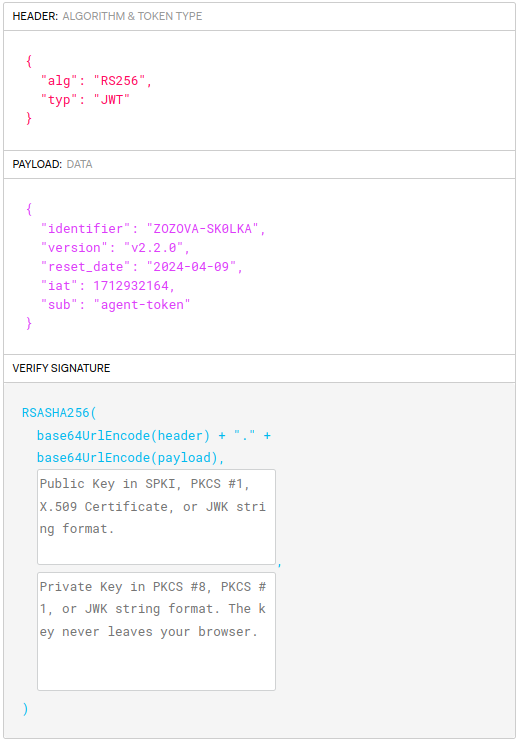
\includegraphics[width=0.5\textwidth]{figures/spaceTraders/jwt.png}
    \caption{Dekódovaný token ze hry SpaceTraders pomocí dekoderu.\cite[JWT decoder]{jwt_decoder}}
    \label{fig:jwt_spacetraders}
\end{figure}

Hra jako první vyžaduje registraci přes endpoint \texttt{/v2/register}. Ten vrátí údaje o novém agentovi spolu s autentizačním tokenem \coderef{code:space_login}[řádek 3]  se kterým se dále bude ověřovat ve všech dalších požadavcích.

\begin{listing}[!ht]
    \inputminted[breaklines]{json}{resources/code/spaceTraders/login.jsonc}
    \caption{Odpověď na požadavek na registraci \protect\footnotemark }
    \label{code:space_login}
\end{listing}
\footnotetext{Velká část dat musela být pro přehlednost smazána}

Jako odpověď používají formát JSON, kde mají vždy objekt \texttt{data} jako objekt zájmu a poté dodatečné objekty jako třeba \texttt{meta} ve kterých může být například stránkování. % TODO odkaz na stránkování
Status odpovědí používají v rámci nepsaných pravidel % TODO odkaz na ty pravidla někde v restku
a dále v obsahu rozšiřují co přesně je na daném požadavku špatně. \coderef{code:space_error}


\begin{listing}[ht!]
    \inputminted[breaklines]{json}{resources/code/spaceTraders/error_response.jsonc}
    \caption{Výpis chyby při požadavku odletět na jinou planetu. (Loď je aktuálně na planetě a není na orbitě. Loď před odletem na jinou planetu musí být na orbitě)}
    \label{code:space_error}
\end{listing}

\section{Specifikace požadavků}
Pomocí analýzy her a vyčlenění požadavků na funkcionality hry(TODO(mám či nemám dávat) od kolegyně) a za pomocí analýzy dostupných nástrojů pro tvorbu API byly vytyčeny požadavky a funkce co by mělo API podporovat. API by mělo podporovat CRUD operace se základními objekty, jejich filtrování, stránkování, a lazy load. API by taktéž mělo podporovat přihlašování a kontrolu před základními typy útoků jako je SQL injection, DDOS a DOS útok a neoprávněný přístup díky chybám v API.

Taktéž by mělo podporovat validaci všech vstupních dat (rozsahy vstupních hodnot, nepovolovat speciální znaky, kontrolovat správný postup operací při hraní hry) a mělo by mít koncové body pro samotné hraní hry.

\subsection{Funkční požadavky}
TODO asi sáhodlouhý výpis funkcionalit?


